\chapter{El reloj de Sol -- II}

\lettrine[lines=2]{A}{ la mañana} siguiente Cecilia se levantó más
temprano que de costumbre; recorría impaciente los interminables
pasillos de Hardvard, pasando una y otra vez por delante de la puerta
cerrada de la oficina de Antonia. Los primeros rayos de Sol ya
atravesaban limpiamente los altos ventanales, trazando en el aire
delicadas, euclídeas y quietas líneas luminosas. Cecilia las
contemplaba y confirmaba su sospecha acerca de la causa del segundo
problema que la desconcertó el día anterior.

Antonia dobló la esquina del largo pasillo que daba a su oficina;
Cecilia, al verla, reprimió un grito de impaciencia y, apoyando los
puños en su cintura, tamborileó ostensiblemente con un pie contra el
piso mientras fruncía el gesto con aire burlón. Antonia, por supuesto,
pareció no darse cuenta de la pequeña farsa urgente, porque mantuvo su
paso tranquilo hasta la puerta de su oficina.

Una vez dentro, y mientras se sentaban frente a la computadora
esperando que Linux preparara la diaria sesión, Cecilia compartió con
Antonia su diagnóstico:

---¿Te acordás de que cuando quisimos agujerear el reloj con todas las
horas desde las 6:00 hasta las 18:00 quitamos de él limpias rebanadas
completas? ---preguntó retóricamente, ya que estaba segura de que
Antonia lo recordaba perfectamente---. Pues bien; creo que ya se
porqué ocurrió  ---y detuvo su discurso con una sonrisa satisfecha,
procurando crear un clima de suspenso.

Antonia la contemplaba en silencio y devolviéndole una sonrisa serena,
por lo que Cecilia, algo mortificada, decidió continuar:

---El giro aparente del Sol alrededor nuestro es muy lento; por esta
razón, las horas que horadamos quedaron muy `pegaditas' una a la otra,
y terminaron por confundir sus cortes entre sí ---y aprovechando que
la computadora mostraba ya operativo el gestor de ventanas, escribió
con rapidez los dos ejemplos de las figuras \ref{fig:13_00} y
\ref{fig:13_01}.

\begin{figure}[ht]
  \begin{minipage}[]{.45\textwidth}
\begin{lstlisting}
module reloj_de_sol(){
 difference(){
  cuerpo(largo_reloj);
  hora_solar(13,0);
 }
}
reloj_de_sol();
\end{lstlisting}%
  \end{minipage}\hfill
  \begin{minipage}[]{.52\textwidth}
    \centering
  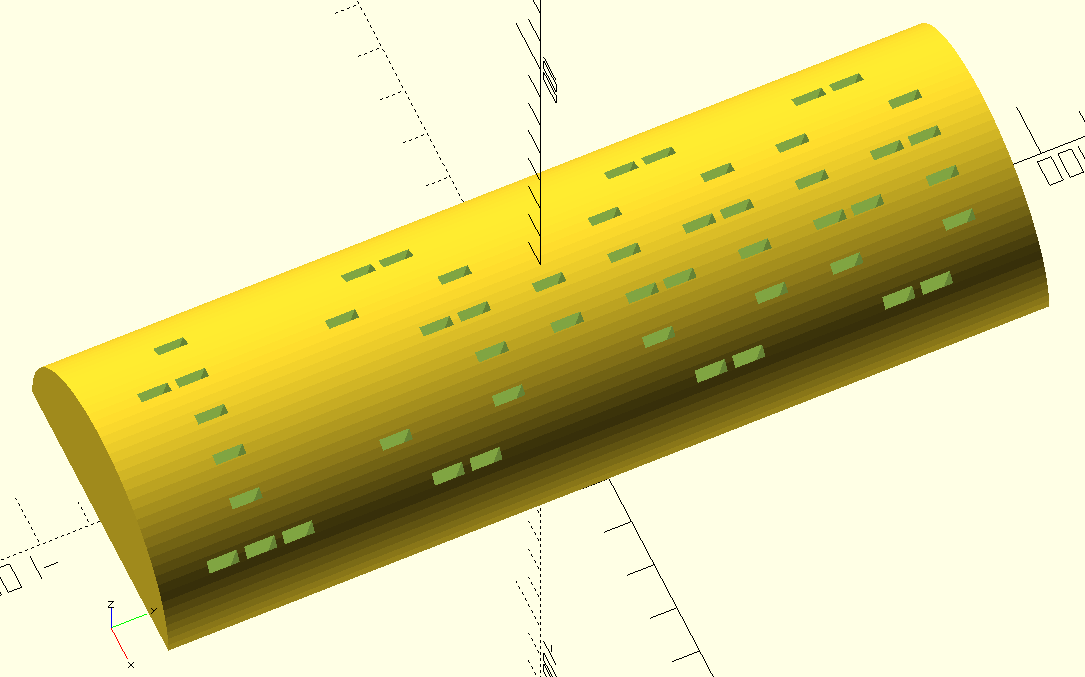
\includegraphics[width=\textwidth]{imagenes/13_00}  
  \end{minipage}
  \caption{Cecilia pretende mostrar que las 13:00...}
  \label{fig:13_00}
\end{figure}

\begin{figure}[ht]
  \begin{minipage}[]{.45\textwidth}
\begin{lstlisting}
module reloj_de_sol(){
 difference(){
  cuerpo(largo_reloj);
  hora_solar(13,1);
 }
}
reloj_de_sol();
\end{lstlisting}%
  \end{minipage}\hfill
  \begin{minipage}[]{.52\textwidth}
    \centering
  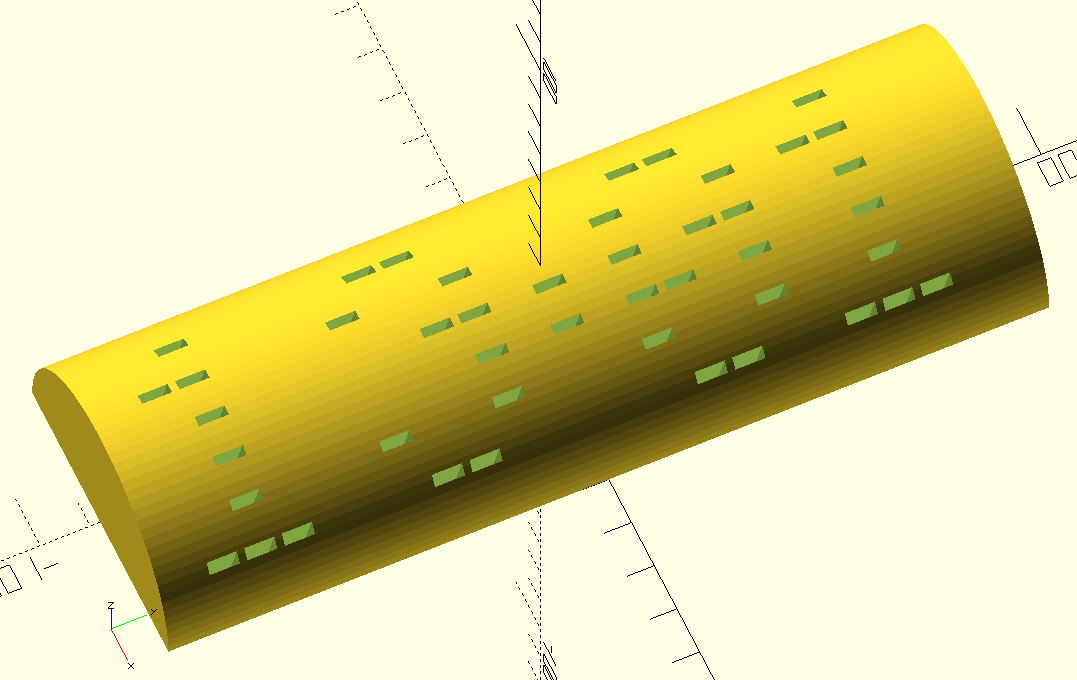
\includegraphics[width=\textwidth]{imagenes/13_01}  
  \end{minipage}
  \caption{...y las 13:01 se encuentran muy cercanas entre sí, y por
    eso se confunden sus cortes.}
  \label{fig:13_01}
\end{figure}

Cecilia no estaba segura de que su punto hubiera quedado claro; de
pronto sintió de manera particularmente intensa la inseguridad que
Antonia debía padecer cuando tenía que explicar casi cualquier cosa.

---Si trato de marcar ambas horas a la vez, se van a confundir entre
sí ---aseguró ahora simulando aplomo mientras escribía otro ejemplo.


\begin{figure}[ht]
  \begin{minipage}[]{.45\textwidth}
\begin{lstlisting}
module reloj_de_sol(){
 difference(){
  cuerpo(largo_reloj);
  hora_solar(13,0);
  hora_solar(13,1);
 }
}
reloj_de_sol();
\end{lstlisting}%
  \end{minipage}\hfill
  \begin{minipage}[]{.52\textwidth}
    \centering
  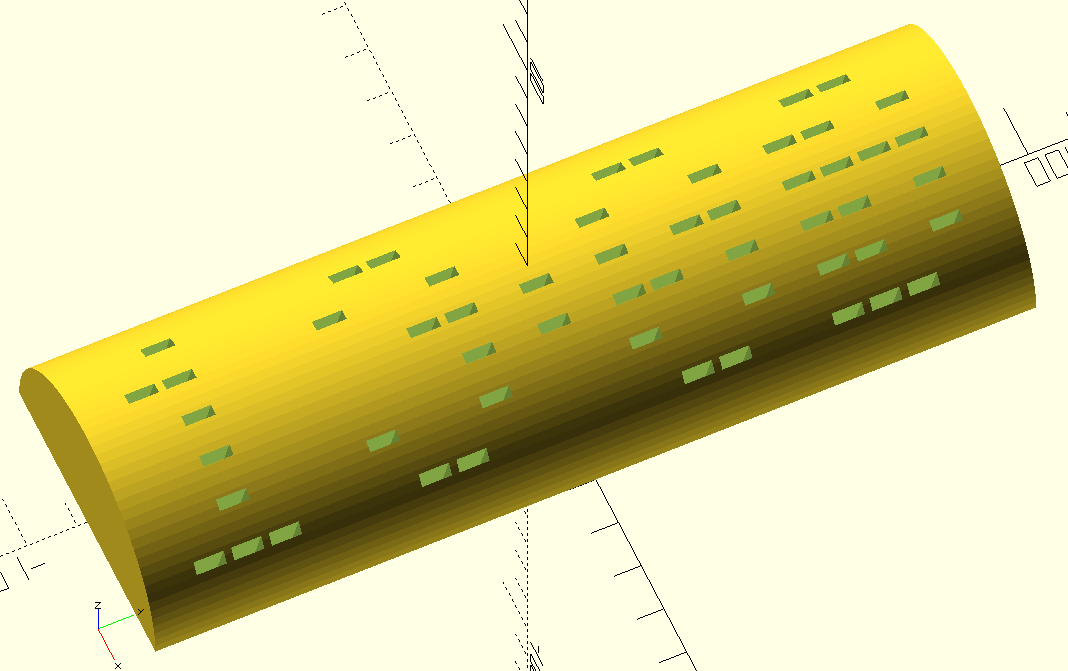
\includegraphics[width=1\textwidth]{imagenes/13_00_01}   
  \end{minipage}
  \caption{Cecilia muestra las 13:00 y las 13:01 a la vez, procurando
    que se aprecie con claridad la confusión que se produce entre
    ambas horas.}
  \label{fig:13_00_01}
\end{figure}


Antonia asintió ahora plenamente y con una amplia sonrisa. Cecilia no
pudo descifrar si aprobaba su conclusión o la manera de exponerla.

---Creo que debemos resignarnos, entonces, a no indicar \emph{todas}
las horas, sino a ciertos intervalos que no se solapen entre sí
---pro\-pu\-so Cecilia.

Antonia expresó su acuerdo marcando aún más su sonrisa; tomó el
teclado para sí y lanzó un <<¡Dale! ¡Probemos!>> que resonó con
entusiasmo en la oficina.

\begin{lstlisting}
module reloj_de_sol(){
  difference(){
    cuerpo(largo_reloj);
    hora_solar(13,0);
    hora_solar(13,10);
  }
}
reloj_de_sol();
\end{lstlisting}%

\begin{figure}[ht]
  \centering
  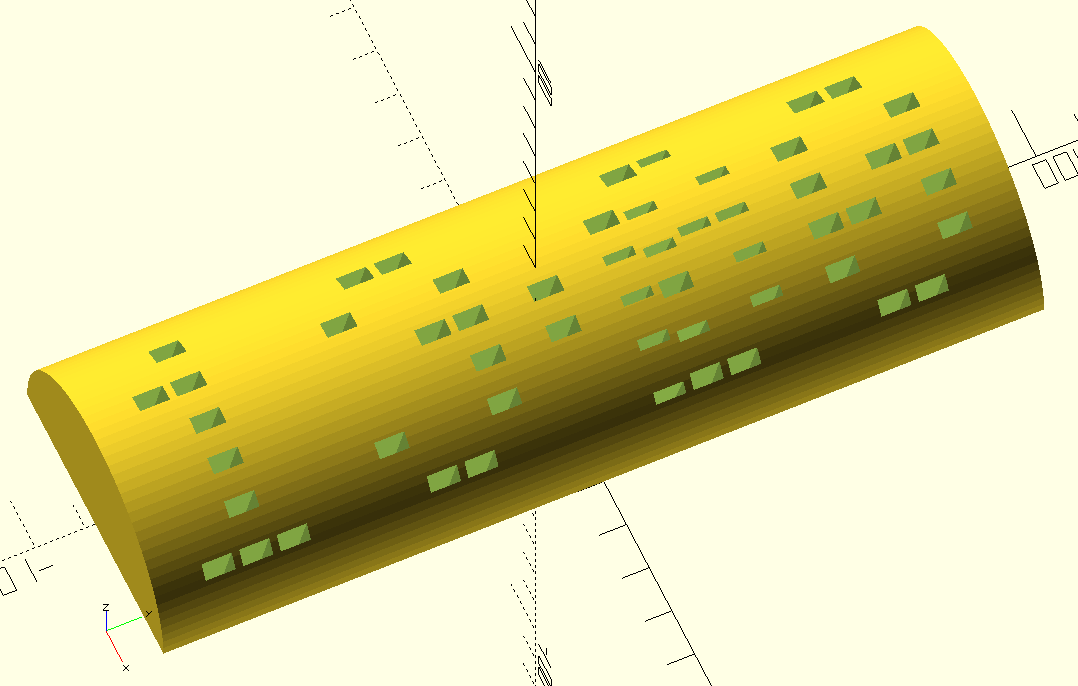
\includegraphics[width=.75\textwidth]{imagenes/13_00_10}  
  \caption{Antonia comprueba que las 13:00 y 13:10 se encuentran aún
    demasiado juntas.}
  \label{fig:13_00_10}
\end{figure}

---Hmmm... parece que 10 minutos sigue siendo un intervalo demasiado
exiguo; probemos con... 20 ---Antonia no disimulaba muy bien su
sobreactuada incertidumbre; Cecilia recordó, además, que su amiga ya
había resuelto e incluso impreso su propio reloj de Sol digital antes
de comenzar el manual. Supuso que, impulsada por su invencible
inclinación didáctica, trataba de recrear para ella los pasos que la
condujeron a la solución. Cecilia no pudo menos que sentir una gran
ternura.

\begin{lstlisting}
module reloj_de_sol(){
  difference(){
    cuerpo(largo_reloj);
    hora_solar(13,0);
    hora_solar(13,20);
  }
}
reloj_de_sol();
\end{lstlisting}%

\begin{figure}[ht]
  \centering
  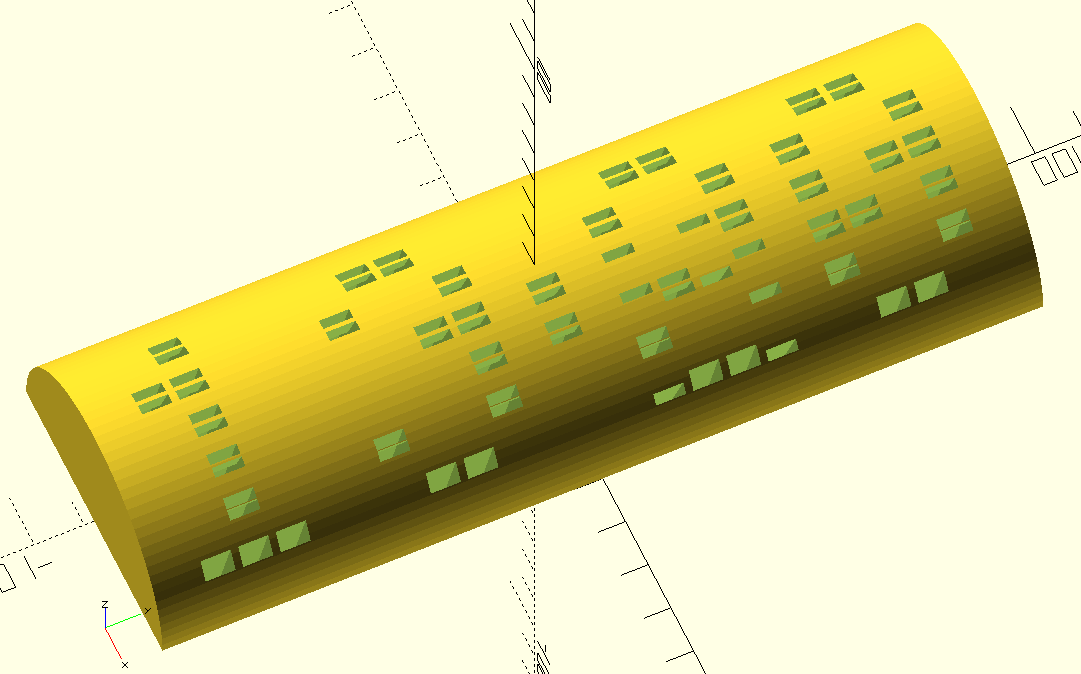
\includegraphics[width=.75\textwidth]{imagenes/13_00_20}  
  \caption{Las 13:00 y las 13:20 parecen distinguirse entre sí.}
  \label{fig:13_00_20}
\end{figure}

---Parece que 20 minutos es un intervalo conveniente ---su\-gi\-rió
Antonia, y Cecilia no pudo estar en desacuerdo.

\section{Rotación del campo de visión}

---¿No te gustaría ver cómo queda cada hora desde la perspectiva del
Sol? ---inquirió Antonia---. Me refiero a poder mirar el reloj desde
la dirección precisa de cada corte; de esa manera, podríamos confirmar
que cada uno resulta bien distinguible del otro.

Cecilia no estaba segura de comprender la pregunta de Antonia, pero en
su tono percibió que era más bien retórica, por lo que con la mirada
la invitó a continuar.

---Voy a tratar de rotar la vista... a ver... ---Antonia se mordía
levemente el labio inferior mientras trataba de hacer puntería con el
ratón; evidentemente, lo suyo era la escritura, y no los dispositivos
apuntadores.


\begin{figure}[ht]
  \centering
  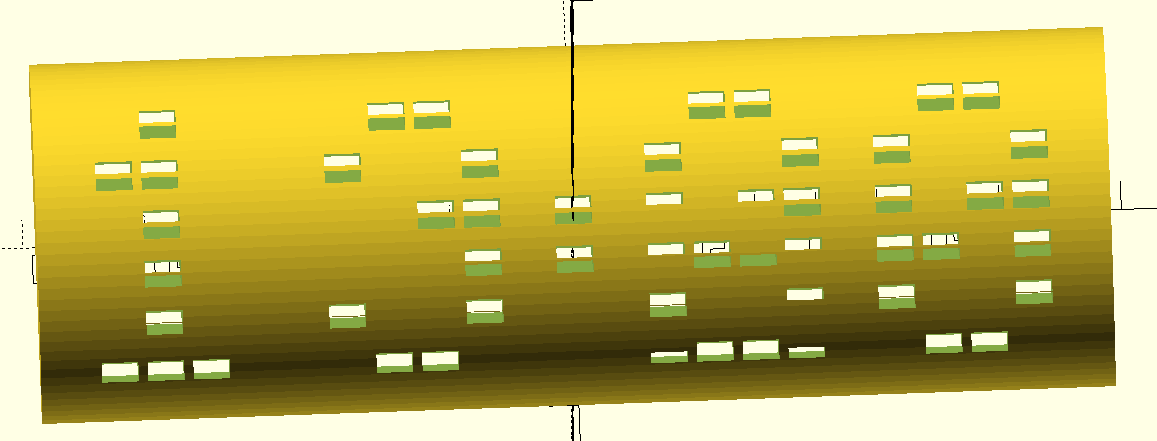
\includegraphics[width=.75\textwidth]{imagenes/vpr-mouse}  
  \caption{Antonia trata en vano de alinear la vista con el ratón.}
  \label{fig:vpr-mouse}
\end{figure}


\guillemotright Por suerte hay una manera de dirigir la mirada por
escrito ---anunció Antonia con tono triunfal; Cecilia comprendió
entonces que toda esa pantomima con el ratón no había sido otra cosa
que uno más de sus trucos infantiles para introducir un tema nuevo, y
exaltar de paso las virtudes de las palabras sobre los demás recursos
expresivos.

\guillemotright La variable del sistema \texttt{\$vpr} sirve para
controlar desde dónde querés ver exactamente la escena; se trata de un
vector que indica dicha dirección. Te confieso que a mí me resulta
bastante difícil deducir, \emph{a priori}, qué valor debe tener para
mostrarme los objetos como quiero ---admitió---; pero hay un truquito
muy útil ---agregó con un guiño---. Fijate abajo a la izquierda.

Cecilia dirigió su mirada a ese extremo del monitor.


\begin{figure}[ht]
  \centering
  
\includegraphics[width=.9\textwidth]{imagenes/vpr-abajo}  
  \caption{La variable \texttt{\$vpr} tiene el valor indicado por la
    etiqueta \texttt{rotate}.}
  \label{fig:vpr-abajo}
\end{figure}



---¿Viste dónde dice \texttt{rotate=[15.70 0.00 87.90]} en la figura
\ref{fig:vpr-abajo}? Ése es el valor que tiene, ahora, la variable
\texttt{\$vpr}. Está claro que esos decimales son los responsables de
la oblicuidad desprolija de la vista que logré, y a duras penas, con
el ratón. Así que no resulta muy difícil deducir cuáles deberían ser
los valores `correctos'.


\begin{lstlisting}
$vpr=[15,0,90];
reloj_de_sol();
\end{lstlisting}%$

\begin{figure}[ht]
  \centering
  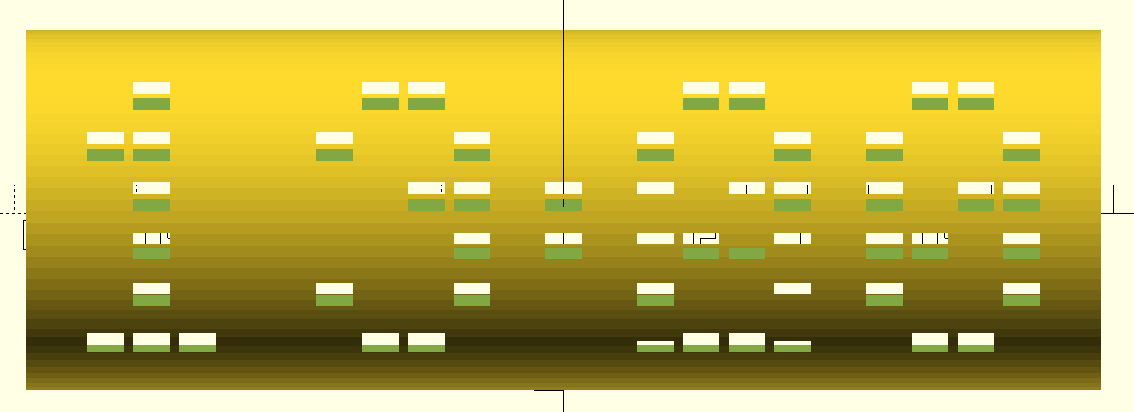
\includegraphics[width=.75\textwidth]{imagenes/vpr_13_00}  
  \caption{Reloj visto desde la dirección de los rayos solares a las
    13:00.}
  \label{fig:vpr_13_00}
\end{figure}

A Cecilia le gustó mucho esa posibilidad:

---Ahora debemos reemplazar el `15' por otro ángulo para poder ver las
13:20 de frente, ¿no? ---preguntó.

---Sí ---confirmó Antonia, pero en su voz sonaba un dejo de
insatisfacción; miraba el monitor como si algo la molestara---.  Quizá
te parezca un tanto quisquillosa, pero me parece que los ejes de la
vista gráfica y los números sobre ellos escritos nos van a molestar un
poco, al interferir con los pixeles. Es muy sutil, pero...

A Cecilia esas marcas no la molestaban en absoluto, pero desde hacía
tiempo sabía que su amiga era muy quisquillosa, y la aceptaba como
era.

Sin esperar su aprobación, Antonia continuó:

---Si desmarcás los botones correspondientes que están sobre la
consola de mensajes, ejes y marcas desaparecerán.


\begin{figure}[ht]
  \centering
  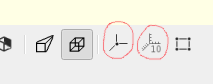
\includegraphics[width=.34\textwidth,valign=c]{imagenes/ejes-marcas}\hfill
  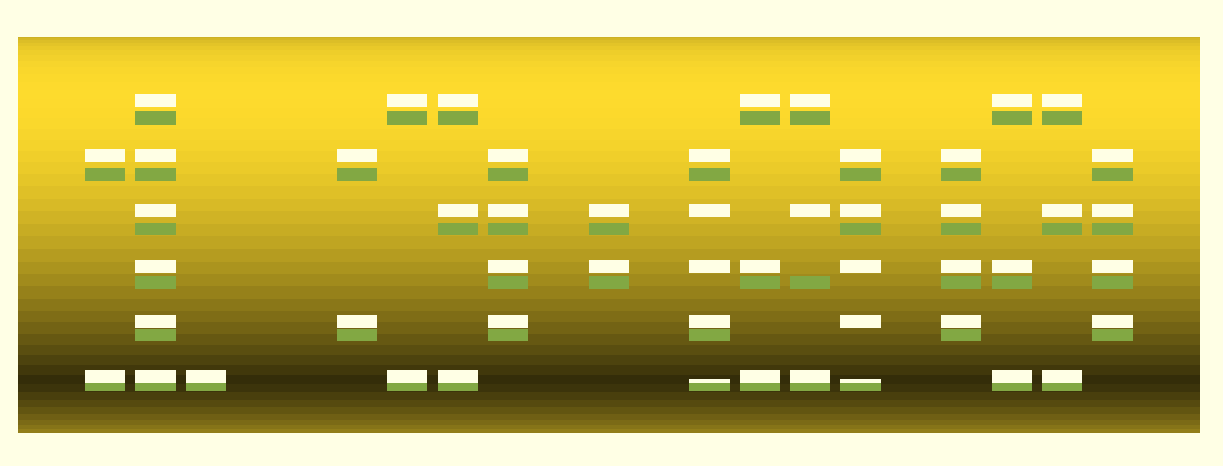
\includegraphics[width=.64\textwidth,valign=c]{imagenes/13_00b}
  \caption{Los ejes de coordenadas y sus marcas pueden ser invisibilizados.}
  \label{fig:ejes-invisibles}
\end{figure}


Ahora, visiblemente más contenta frente a la figura
\ref{fig:ejes-invisibles}, Antonia prosiguió:

---Como decías, ahora debemos cambiar el `15' por otro ángulo, pero en
lugar de calcularlo vamos a dejar que \openscad{} lo haga por nosotras
---y acompañó esta propuesta con otro de sus infaltables guiños.


\begin{lstlisting}
$vpr=[90-alfa(13+20/60),0,90];
reloj_de_sol();
\end{lstlisting}%$

\begin{figure}[ht]
  \centering
  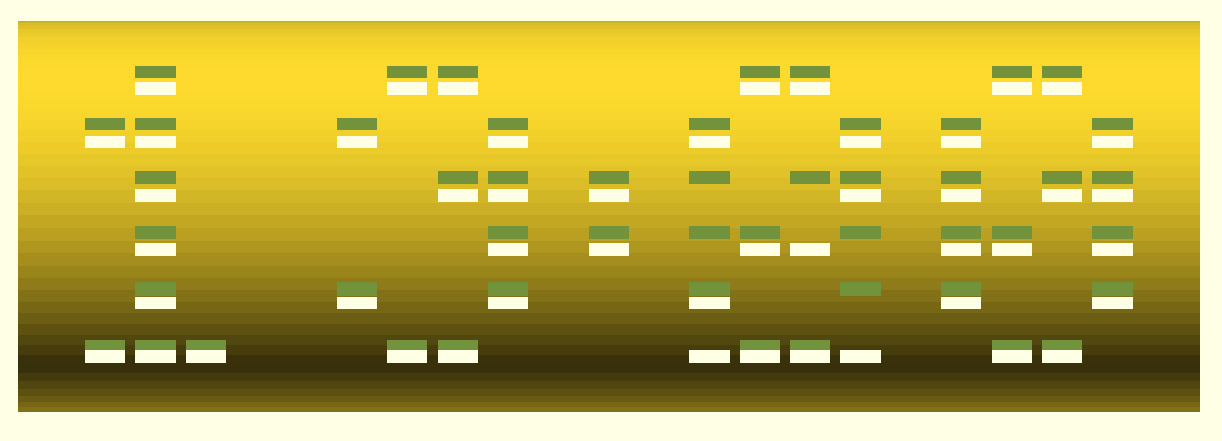
\includegraphics[width=.75\textwidth]{imagenes/vpr_13_20}  
  \caption{Reloj visto desde la dirección de los rayos solares a las
    13:20.}
  \label{fig:vpr_13_20}
\end{figure}

Cecilia no pudo evitar ceder a la pulsión por comprender; con los ojos
entornados observó atentamente el texto. Le pareció que el `90'
ubicado en la tercera posición del vector de
\texttt{\$vpr} representaba la rotación de la vista alrededor del eje
\coord{Z}: quizá gracias a ella estaban viendo el reloj
``horizontalmente'' en relación al monitor. Por su parte, el valor que
ocupaba el primer lugar en el vector tal vez determinaba la rotación
en torno al eje \coord{X}, que coincidía con el eje principal del
reloj. Dicho ángulo se obtenía restando de 90 el que devolvía la
función \lstinline!alfa! que habían escrito, capítulos antes, con
Antonia: tal vez esa resta se debía a que ellas medían los ángulos
desde las 12:00, mientras que \openscad{} seguramente lo haría desde
el plano \coord{XY}.

Antonia sacó a Cecilia bruscamente de sus cavilaciones:

---¿No tenés ganas de agujerear más horas? ---preguntó, mientras
escribía.


\begin{lstlisting}
module reloj_de_sol(){
  difference(){
    cuerpo(largo_reloj);
    hora_solar(12,0);
    hora_solar(12,20);
    hora_solar(12,40);
    hora_solar(13,0);
    hora_solar(13,20);
    hora_solar(13,40);
  }
}
reloj_de_sol();
\end{lstlisting}%

\begin{figure}[ht]
  \centering
  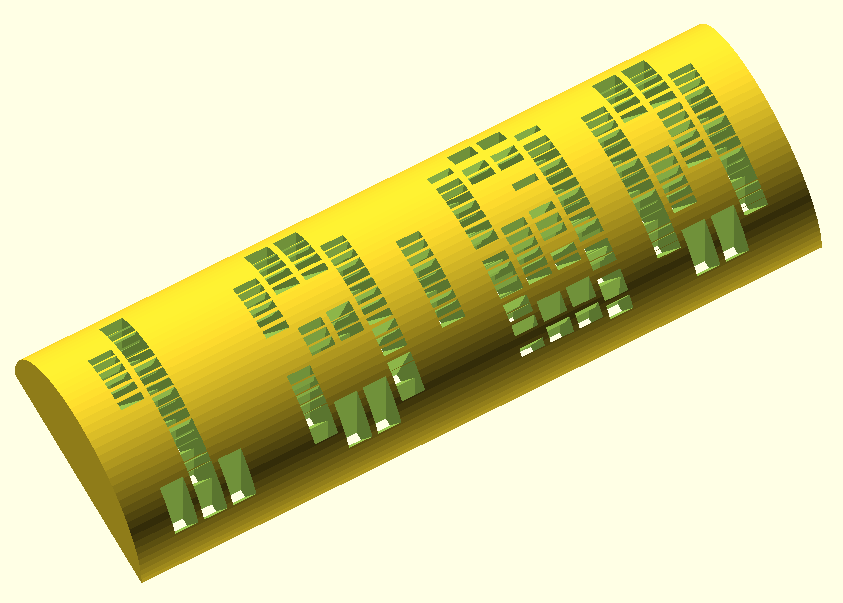
\includegraphics[width=.97\textwidth]{imagenes/12_00_13_40}  
  \caption{Reloj horadado con las horas que van desde las 12:00 a las
    13:40 en intervalos de 20 minutos.}
  \label{fig:12_00_13_40}
\end{figure}

\section{Animaciones}

Cecilia se sentía cada vez más entusiasmada y feliz. La compilación de
las seis horas elegidas llevó su tiempo en la computadora de Antonia,
pero le parecía razonable: se trataba de varios orificios. Por lo
demás, después de
\setcounter{m}{\thechapter}\addtocounter{m}{0}\them{} capítulos de
pésima literatura y poco rigurosa exposición técnica se sentía
perfectamente capaz de esperar unos cuantos minutos más.

---Ahora podríamos ver el reloj desde cada una de las horas perforadas
---el tono de Antonia era inequívoco: indudablemente estaba por
proponer algo que creía mucho mejor que eso---. Pero... ¿no te
gustaría que \openscad{} rotara animadamente el reloj ante tus ojos
para que pudieras apreciar la suave transición de las horas?

Cecilia los abrió desmesuradamente: ¿Sería posible? Inmediatamente
comprendió que sí; a esta altura, ya nada la sorprendía del ingenio de
los creadores de este lenguaje.

---Empecemos por un ejemplo... elemental ---dijo Antonia, aunque
Cecilia tradujo para sus adentros ese término con un seguramente más
apropiado ``tonto''.

\begin{lstlisting}
rotate([0,0,$t*360])
  cube([30,30,2],center=true);
  
translate([40,0,0])
  rotate([0,0,-$t*360])
    cube([20,20,2],center=true);
\end{lstlisting}%

\begin{figure}[ht]
  \centering
  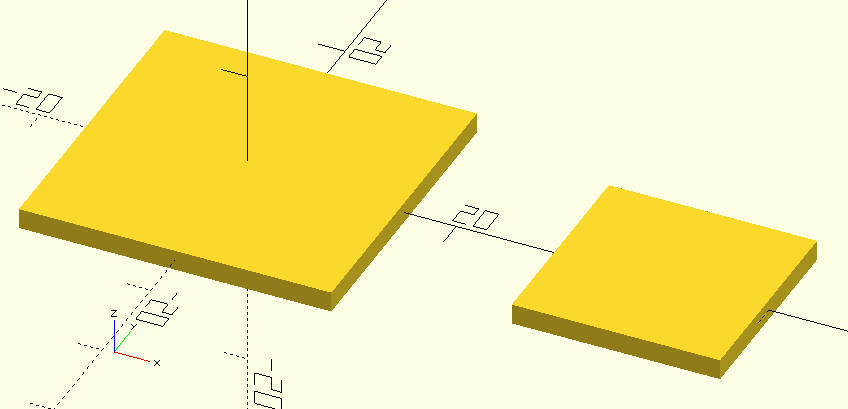
\includegraphics[width=.55\textwidth]{imagenes/animacion-0}  
  \caption{Cubos dispuestos para ser animados por \openscad.}
  \label{fig:animacion-0}
\end{figure}

\guillemotright Como podrás apreciar, en principio escribí dos simples
cubos. Bueno, está bien: ortoedros ---aclaró a
re\-ga\-ña\-dien\-tes---. Pero fijate que en las rotaciones de las
líneas 1 y 5 aludo a una extraña variable aparentemente no definida:
\texttt{\$t} ---Antonia puso cara de misterio antes de proseguir---. Y
\openscad{} ni chistó: la figura \ref{fig:animacion-0} parece indicar que
la conoce.

Cecilia se preguntaba en silencio hasta cuándo su amiga iba a dilatar
ineficazmente el suspenso.

---Pues bien, resulta que \texttt{\$t} es otra variable más del
sistema.  Representa el tiempo: ese gran misterio que deslumbró y
sigue atareando a los más diversos filósofos y artistas; esa materia
de la que, al decir de Borges, estamos hechos ---el tono de Antonia
adquirió, quizás a su pesar, un cierto tono vibrante. Cecilia hizo un
esfuerzo por reprimir un bostezo.

---Si ahora hacés \emph{click} en la entrada del menú \texttt{Ver}
$\rightarrow$ \texttt{Animar}, vas a notar que sobre la consola
aparecen mágicamente tres nuevos cuadros de texto: \texttt{Tiempo},
\texttt{FPS} y \texttt{Pasos}.

\begin{figure}[ht]
  \centering
  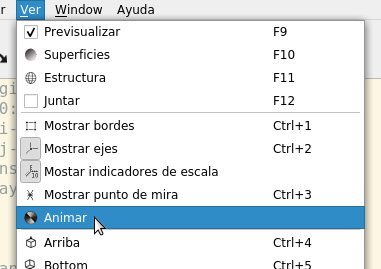
\includegraphics[width=.5\textwidth]{imagenes/animar-menu}
  
  \vspace{1ex}
  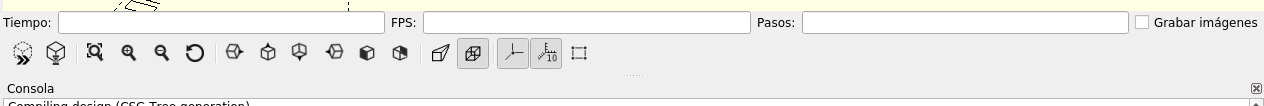
\includegraphics[width=1\textwidth]{imagenes/animar-cuadros}
  \caption{El menú \texttt{Animar} permite la animación de las escenas
    de \openscad.}
  \label{fig:menu-animar}
\end{figure}
  

\guillemotright En el cuadro \texttt{Tiempo} no escribas nada; su
función exclusiva consiste en mostrar el avance del mismo, de 0 a 1 y
vuelta a empezar desde 0, cíclicamente, en intervalos de 0,01
---explicó Antonia y se detuvo un momento, mientras dirigía una mirada
ensoñadora al techo---. Las hermosas paradojas de Zenón de Elea no
hubieran alarmado nuestra juventud si el tiempo fuera tan
ostensiblemente granular ---y suspiró con una melancólica sonrisa.

\guillemotright Los cuadros para los que sí es necesario decidir
valores son los otros dos ---Antonia retomó no sin esfuerzo su
explicación---. En \texttt{FPS} debés indicar la velocidad con la que
querés que se desarrolle la animación (FPS, como sin duda sabrás, son
las siglas de \emph{Frames Per Second}: cuadros por segundo, en
inglés): un valor más alto representa una velocidad mayor. Por su
parte, en \texttt{Pasos} debés señalar en cuantos `cuadros'
(\emph{Frames}) querés dividir el intervalo de tiempo completo de 0 a
1. Por ejemplo, si ponemos 5 en \texttt{FPS} y 100 en \texttt{Pasos},
la animación discurrirá a una velocidad de 5 cuadros por segundo (una
suerte de `cámara lenta') y la rotación completa se realizará por
saltos de 3,6$^{\circ}$ (360$^{\circ}$/100), porque la rotación avanza según
\texttt{\$t*360}: fijate las líneas 1 y 5 del ejemplo.

A Cecilia le pareció mucha información junta, y la explicación de
Antonia ---como siempre--- no era de la mayor eficacia; decidió una
vez más que la mejor manera de aprehender este nuevo concepto sería
probarlo y escribirlo varias veces por su propia cuenta en ejemplos
diversos.

---Si en lugar de cubos hubiéramos escrito engranajes, la animación
sería bastante más interesante ---reflexionó Antonia, con un dejo de
resignación---. Pero en fin; veamos cómo aplicar las animaciones a la
rotación del campo de visión.

\guillemotright En principio y en nuestro ejemplo, queremos que la
rotación abarque desde las 12:00 hasta las 13:40. Por un lado, para
mirar de frente a las 12:00, \texttt{\$vpr} debe valer
\lstinline![0,0,90]!, y para las 13:40 debe ser igual a
\lstinline![25,0,90]!, porque \lstinline!90-alfa(13+40/60)=25!
---dijo, mientras escribía los ejemplos de las figuras
\ref{fig:animacion_12_00} y \ref{fig:animacion_13_40}.




\begin{figure}[ht]
  \begin{minipage}[]{.3\textwidth}
\begin{lstlisting}
$vpr=[0,0,90];
reloj_de_sol();
\end{lstlisting}%$
  \end{minipage}\hfill
  \begin{minipage}[]{.68\textwidth}
    \centering
    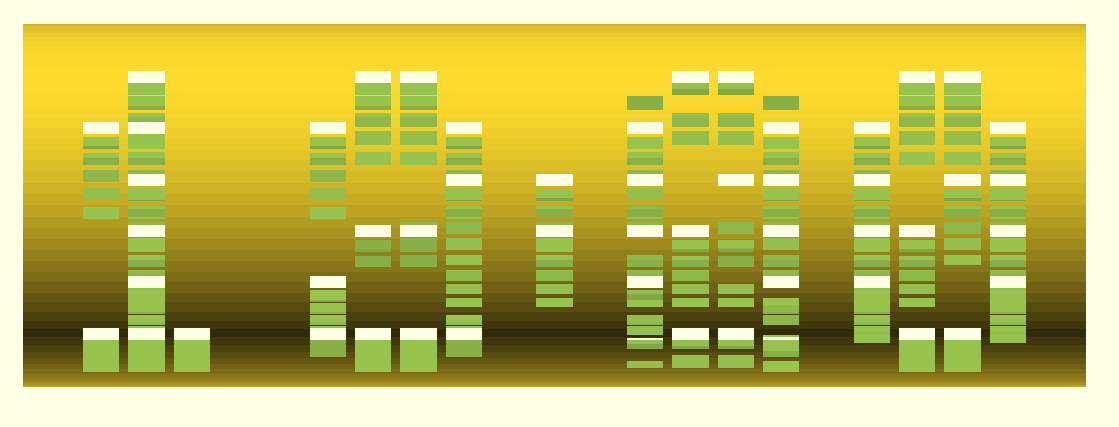
\includegraphics[width=1\textwidth]{imagenes/animacion_12_00}  
  \end{minipage}
    \caption{Para ver de frente las 12:00, \texttt{\$vpr=[0,0,90]}.}
  \label{fig:animacion_12_00}
\end{figure}



\begin{figure}[ht]
  \begin{minipage}[]{.3\textwidth}
\begin{lstlisting}
$vpr=[25,0,90];
reloj_de_sol();
\end{lstlisting}%$
  \end{minipage}\hfill
  \begin{minipage}[]{.68\textwidth}
    \centering
  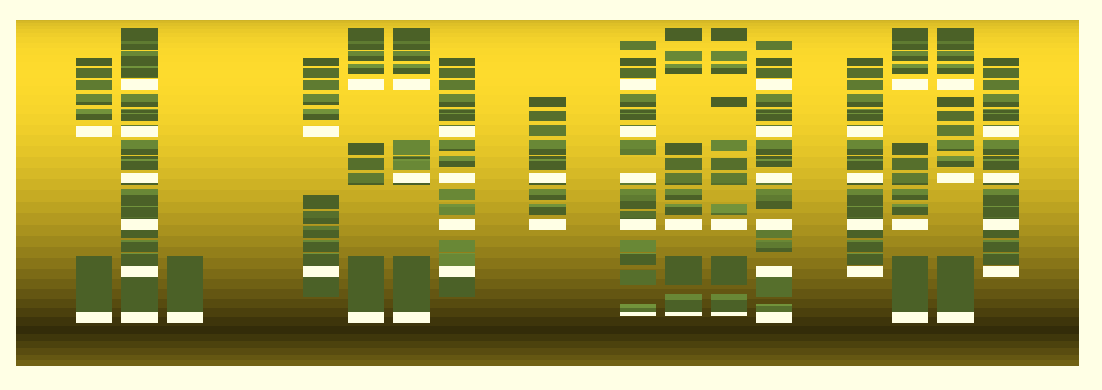
\includegraphics[width=1\textwidth]{imagenes/animacion_13_40}  
  \end{minipage}
  \caption{Para ver de frente las 13:40, \texttt{\$vpr=[25,0,90]}.}
  \label{fig:animacion_13_40}
\end{figure}




\guillemotright Así que necesitamos que para \texttt{\$t=0} sea
\texttt{\$vpr=[0,0,90]}, y para \texttt{\$t=1} sea
\texttt{\$vpr=[25,0,90]}. Creo que la conclusión es inmediata
---expresó Antonia con su invencible optimismo.

\begin{lstlisting}
$vpr=[$t*25,0,90];
reloj_de_sol();
\end{lstlisting}%

Antonia empleó 2 y 40 para \texttt{FPS} y \texttt{Pasos},
respectivamente. A Cecilia le gustó la animación, pero algo la
inquietó súbitamente:

---Antonia... en la imagen \ref{fig:animacion_13_40} puedo ver algunos
pixeles `medio encendidos' debajo del 4...

Antonia frunció los labios mientras asentía levemente:

---Sí... es verdad ---admitió---. Es un problema. Para evitarlo se me
ocurren dos caminos: hacer los pixeles menos altos, o separar más las
horas entre sí. Ninguna de las soluciones me satisface del todo:
señalar las horas cada 30 minutos relega nuestro reloj a un estado
casi testimonial, por así decirlo; y pixeles muy delgados podrían
atentar contra la legibilidad de la hora.

Tras unos instantes en que ambas amigas dudaban frente al monitor,
evaluando incluso la posibilidad de dejar todo como estaba, Cecilia se
decidió a probar la primera opción:

\begin{lstlisting}[numbers=none]
alto_pixel = 1.6; // era 2
\end{lstlisting}%

\begin{figure}[ht]
  \centering
  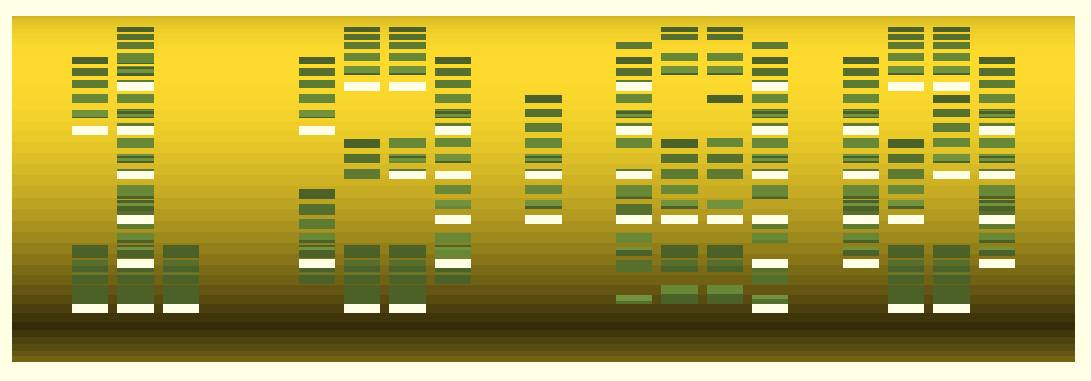
\includegraphics[width=.8\textwidth]{imagenes/13_40_1_6}  
  \caption{Cecilia prueba la posibilidad de que
    \texttt{alto\_pixel=1.6}.}
  \label{fig:13_40_1_6}
\end{figure}


---No está mal; yo diría que lo dejemos así ---propuso An\-to\-nia
contemplando la figura \ref{fig:13_40_1_6}---. Y con respecto a la
animación, a los lectores se las debo; incrustar un gif animado en un
pdf no siempre funciona, y en todo caso torna muy grande el archivo
resultante ---se excusó.

---¿Y no te parece una pena que no la puedan ver..?  ---pre\-gun\-tó
Cecilia.

Antonia se encogió de hombros:

---Sinceramente, no puedo imaginar un lector de este manual que haya
llegado a la página \thepage{} y no tenga \openscad{} a la mano
---a\-fir\-mó, y casi inmediatamente, añadió---: De hecho, casi no
puedo imaginar ningún tipo de lector para este manual.

Cecilia no pudo evitar estar de acuerdo.


%%% Local Variables:
%%% mode: latex
%%% TeX-master: "../libro"
%%% End:
